\documentclass{article}

\usepackage{times}
\usepackage{graphicx}
\usepackage{url} % for typesetting urls
\usepackage{color}
\usepackage{fancybox}
\usepackage{amssymb}
\usepackage{amsmath}
\usepackage{framed}
%\usepackage{hyperref}
\usepackage[super,square]{natbib}
\usepackage[a4paper,lmargin=35mm,tmargin=35mm,bmargin=35mm,rmargin=35mm,twoside=false,marginpar=30mm]{geometry}

% ------------------------------------------------------------------------
\definecolor{lightgray}{RGB}{225,225,225}

\newenvironment{eg}{\par\noindent{\bf Example.}}{\hfill$\blacksquare$}
\newenvironment{insight}[1]{
\begin{framed}
\noindent\begin{minipage}[t]{0.05\textwidth}
{\Huge ?}
\end{minipage}%
\begin{minipage}[m]{0.95\textwidth}
{\bf #1}
}{\end{minipage}\end{framed}}

% ------------------------------------------------------------------------

\usepackage{listings}

% ==========================================
% Whiley LstListing Mode
% ==========================================

\pagestyle{plain}
\lstloadlanguages{Java}
\lstset{
        language=Java,
        keywords={function, method, type, constant, assert, for, while, switch, is, if, case, return,
          else, process, define, as, requires, ensures, where, no, new,
          all, bool, int, byte, char, string, void, real, in, any,
          null, var, public, protected, private
        },
        basicstyle=\small\ttfamily,
        commentstyle=\rmfamily\itshape,
        %%Uncomment the following line to avoid boldface keywords
        % keywordstyle=\ttfamily,
        stringstyle=\small\itshape,
        moredelim=*[s][commentstyle]{/*}{*/}, % allows keyword highlighting inside comments
        morecomment=[l][commentstyle]{//},      % single line comments are set by...
        backgroundcolor=\color{lightgray},
        frame=single, % adds a frame around the code
%        frameround=tttt,
        framesep=0.25cm,
        texcl,                                                          % ...LaTeX
        moredelim=[is][\ttfamily]{<code>}{</code>}, % allows setting code inside multi-line comments
        moredelim=*[s][\ttfamily]{/*@}{*/}, % JML annotations
        moredelim=*[l][\ttfamily]{//@}, % JML annotations
        moredelim=**[is][\itshape]{/_}{_/}, % allows emphasizing sub-expressions
        moredelim=**[is][\bfseries]{/b_}{_b/}, % allows emphasizing sub-expressions
        escapeinside={(*@}{@*)}, %use (*@\label{line:desc}@*) to label lines for \ref
        mathescape=true,                % allow $ $ for math mode (will this break things?}
        tabsize=4,
	tab=\rightarrowfill,
        xleftmargin=0.25cm,
        xrightmargin=0.25cm,
        showspaces=false,
        showtabs=false,
        columns=fullflexible,
        numberstyle=\tiny,
        keepspaces=true,
        mathescape=true, % allows $ to switch in and out of math mode within listings
        literate={->}{{$\rightarrow$}}1 
           {tau}{{$\tau$}}1 {tau'}{{$\tau\prime$}}1 {(|}{{$\lpbar$}}1 {---}{{$\hole$}}1
           {-*-}{{$\times$}}1 {||_}{{$\lceilfloor$}}1 {_||}{{$\rceilfloor$}}1
           {/0}{{$\emptyset$}}1 {/bul}{{$\unit$}}1 {:->}{{$\mapsto$}}1
           {~}{$\sim$}1,
}


\title{\Huge Getting Started with Whiley}

\author{David J. Pearce}

\begin{document}
\maketitle
\begin{abstract}
  The aim of this document is to provide a short introduction to the
  Whiley programming language, in order to get you up and running
  quickly.  However, it is not intended to be a definitive reference.
  We'll walk through a number of simple examples illustrating the most
  interesting features of Whiley, and show you how to get it up and
  running.  We will be assuming some rudimentary knowledge of
  programming.
\end{abstract}
\tableofcontents
\clearpage
\chapter{Introduction}
When we write software, we have in mind some idea of what it is supposed to do.  When we've finished our program, we might run it to see whether it appears to do the right thing.  However, as anyone who has ever written a program will know: {\em this is not always enough!}  Even if our program appears to work after a few tests, there is still a good chance it will go wrong for other inputs we have not yet tried.  The question, then, is: {\em how can we be certain that our program is correct?}

In trying to determine whether our program is correct, our first goal is to determine precisely what it should do.  In writing our program, we may not have had a clear idea of this from the outset.  Therefore, we need to determine a {\em specification} for our program.  This is a precise description of what the program should and should not do.  Only with this can we begin to consider whether or not our program actually does the right thing.


\section{Infamous Software Failures}

Introduce some classic historical bugs, and emphasis that we want to reduce these as much as possible.  There are lots of good examples, some of which are not coding failures but failures of understanding the requirements, etc.

Numerous important software systems have failed due to program bugs. Historic examples include the Therac-25 disaster where a computer-operated X-ray machine gave lethal doses to patients, the 1988 worm which wreaked havoc on the internet by exploiting a buffer overrun, and the (unmanned) Ariane 5 rocket which exploded shortly after launch because of an integer overflow (see this video and this list for more).

\section{Programming Languages}

Modern programming languages, such as Java and C\#, eliminate fairly simple classes of error (so-called type errors) through the process of type checking; however, they cannot detect more complex problems, such as the potential for a divide-by-zero error. Type checking has been used for a long time in programming languages, historical examples of which include: ALGOL, Pascal, Modula-2, C, C++, Java, C\# and more.

\section{Whiley}
The Whiley programming language has been in active development since
2009.  The language was designed specifically to help the programmer
eliminate bugs from his/her software.  The key feature is that Whiley
allows programmers to write {\em specifications} for their functions,
which are then checked by the compiler.  For example, here is the
specification for the \lstinline{max()} function which returns the
maximum of two integers:

\begin{lstlisting}
function max(int x, int y) => (int z)
// must return either x or y
ensures x == z || y == z
// return must be as large as x and y
ensures x <= z && y <= z:
    // implementation
    if x > y:
        return x
    else:
        return y
\end{lstlisting}

Here, we see our first piece of Whiley code.  This declares a function
called \lstinline{max} which accepts two integers \lstinline{x} and
\lstinline{y}, and returns an integer \lstinline{z}.  The body of the
function simply compares the two parameters and returns the largest.
The two \lstinline{requires} clauses form the function's {\em
  post-condition}, which is a guarantee made to any caller of this
function.  In this case, the \lstinline{max} function guarantees to
return one of the two parameters, and that the return will be as large
as both of them.  In plain English, this means it will return the
maximum of the two parameter values.

When verification is enabled the Whiley compiler will check that every
function meets its specification.  For our \lstinline{max()} function,
this means it will check that body of the function guarantees to
return a value which meets the function's post-condition.  To do this,
it will explore the two execution paths of the function and check each
one separately.  If it finds a path which does not meet the
post-condition, the compiler will report an error.  In this case, the
\lstinline{max()} function above is implemented correctly and so it
will find no errors.  The advantage of providing specifications is
that they can help uncover bugs and other, more serious, problems
earlier in the development cycle.  This leads to software which is
both more reliable and more easily maintained (since the
specifications provide important documentation).

\subsection{Objectives}

\newpage
\section{Quick Walkthrough}
This section provides a quick walk through of the main concepts and
ideas in the Whiley language.  Through a series of short examples,
we'll introduce the basic building blocks of the language.

\subsection{Booleans and Numbers}

As found in many languages, Whiley supports a range of primitive
datatypes for representing boolean, integers, real numbers, bytes,
characters, etc.  Of these, the most commonly used are:

\begin{itemize}
\item {\bf Booleans} are denoted by the type \lstinline{bool}.  This is the
  simplest of the primitive datatypes, and has only two possible
  values: \lstinline{true} or \lstinline{false}.
\item {\bf Integers} are denoted by the type \lstinline{int}.  Integers in
  Whiley are {\em unbounded}. This means that, in theory at least, a
  variable of type int can take on {\em any possible integer value};
  this differs from many other languages (e.g. Java), which limit the
  number of possible values (e.g. following 32-bit two's complement).
\item {\bf Real Numbers} are denoted by the type
  \lstinline{real}. Reals in Whiley are {\em unbounded
    rationals}. This means that, in theory at least, a variable of
  type real can take on {\em any possible rational value}. Again, this
  offers significantly better precision than, for example,
  \lstinline{float} or \lstinline{double} types based on IEEE754 as
  found in other languages (e.g. Java).
\end{itemize}


\noindent A very simple example which illustrates the \lstinline{int} and
\lstinline{bool} types is the following:

\lstinputlisting{../examples/walkthrough_1.whiley}

This declares a simple function which returns \lstinline{true} if the
first parameter, \lstinline{x}, is less than the second,
\lstinline{y}, and \lstinline{false} otherwise.

\begin{insight}{Indentation Syntax.}
  From the above example you should notice that Whiley, unlike many
  languages, does not use curly braces (i.e. \verb+{ ... }+) to
  demarcate blocks of code.  Instead, Whiley uses {\em indentation
    syntax} which was popularised by the Python programming language.
  The start of a new code block is signalled by a preceding \verb+:+
  on the previous line.  The new block must be indented by at least
  one space (the actual amount doesn't matter) and all subsequent
  statements with the same indentation are included.
\end{insight}

\begin{insight}{Ints versus Reals.}
Unlike many other languages, Whiley provides a strong relationship
between values of type \lstinline{int} and those of type
\lstinline{real}.  Specifically, every \lstinline{int} value can be
represented precisely as a \lstinline{real} value.  Although it may
seem surprising, this is not true for many other languages
(e.g. Java), where there are \lstinline{int} (resp. \lstinline{long})
values which cannot be represented using \lstinline{float}
(resp. \lstinline{double})~\cite{GJSB05}.
\end{insight}

% \begin{lstlisting}
% function floor(real x) => int:
%     int num / int den = x    // extract numerator and denominator
%     int r = num / den        // integer division
%     if x < 0.0 && den != 1: 	 
%         return r - 1 
%     else:
%         return r 
% \end{lstlisting}

\newpage
\subsection{Sets, Lists and Maps}
\label{walkthrough_collections}
Like many modern programming languages, Whiley provides built-in types
for representing collections.  The following illustrates a short
function which multiplies a vector by a scalar:

\lstinputlisting{../examples/walkthrough_2.whiley}

This illustrates a few of the common collection operations.  Firstly,
the size of a collection is obtained using the {\em length} operator
(i.e. \lstinline{|vector|} returns the length of \lstinline{vector}).
Secondly, the \lstinline{for} loop is useful for iterating over the
elements of a collection.  In this case, \lstinline{0 .. |vector|}
returns a {\em list} of consecutive integers from \lstinline{0} up to
(but not including) \lstinline{|vector|}.  Finally, the {\em list
  access} operator, \lstinline{vector[i]}, returns the element at
index \lstinline{i}.  The three different kinds of collections
supported in Whiley are:
\begin{itemize}
\item {\bf Sets} (e.g. \lstinline|{int}|) provide the simplest form of collection, and are constructing using a {\em set constructor} (e.g. \lstinline|{1,2,3}|).  They support the {\em set union} (e.g. \lstinline{xs + ys}), {\em set intersection} (e.g. \lstinline{xs & ys}) and {\em set difference} (e.g. \lstinline{xs - ys}) operators.  One can test for inclusion using the {\em element of} operator (e.g. \lstinline{x in xs}), or the {\em subset} (e.g. \lstinline{xs $\subset$ ys}) and {\em subset or equal} (e.g. \lstinline{xs $\subseteq$ ys}) operators.
  
\item {\bf Maps} (e.g. \lstinline|{int=>string}|) provide a halfway point between sets and lists.  They are similar to dictionaries in Python or the \lstinline{Map} interface in Java.  They can be viewed as a set of {\em key$\times$ value} pairs, where every key maps to exactly one value.  Maps are constructed using a {\em map constructor} (e.g. \lstinline|{1=>"hello",2=>"world"}|), and elements are accessed using the {\em map access} operator (e.g. \lstinline{map[i]}).  

\item {\bf Lists} (e.g. \lstinline{[int]}) are similar to arrays
  (e.g. in Java), but they can also be resized.  As can be seen above,
  they support the {\em list access} operator
  (e.g. \lstinline{vector[i]}).  They also support the {\em list
    append} operator (e.g. \lstinline{[1,2,3] ++ [4,5,6]}) and {\em
    sublist} operator (e.g. \lstinline{vector[0..2]}).  Finally, lists are constructed using a {\em list constructor} (e.g. \lstinline{[1,2,3]}).

\end{itemize}

All collection kinds can be iterated using the built-in
\lstinline{for} loop construct.  For example, here is a function to iterate a map looking for a particular value:

\lstinputlisting{../examples/walkthrough_3.whiley}

\noindent This function iterates over each key$\times$value pair (i.e. \lstinline{k,v}) in a from integers to strings (i.e. \lstinline|{int=>string}|) using the \lstinline{for} statement.

\subsection{Records and Tuples}
Aside from collection types, Whiley also allows provides {\em records} and {\em tuples} for grouping items together.  Records are similar to \lstinline{struct}s (as found in C) and objects (as found in JavaScript).  A record is constructed from one or more {\em fields}, each of which has a unique name and type.  For example, the following defines a simple record type for representing 2D points and a function for translating their position:

\lstinputlisting{../examples/walkthrough_4.whiley}

Here, a {\em user-defined type} named \lstinline{Point} has been defined.  This is a record type containing two \lstinline{int} fields, \lstinline{x} and \lstinline{y}.  In the \lstinline{translate()} function, a {\em record literal} is used to construct a new \lstinline{Point} to be returned.

Records are an important mechanism for giving meaning to data in Whiley.  For example, consider the following declaration of a rectangle:

\lstinputlisting{../examples/walkthrough_5.whiley}

Here, we see that a rectangle has a position, a width and a height.  The names of the fields are important for conveying their meaning in the real-world.

Sometimes, using a record type is a little more than necessary because the data being described is really quite simple.  In such cases we can use a {\em tuple} in Whiley, which provide a lightweight mechanism for grouping data.  For example, we might consider that using a record to defined our \lstinline{Point} is a little verbose.  Instead, we could rework the example to use a tuple as follows:

\lstinputlisting[firstline=4]{../examples/walkthrough_6.whiley}

Since there is a widely used notation for describing 2D points --- namely $(x,y)$ --- it makes sense in this case to use a tuple over a record.  Tuples are also useful for describing functions which return multiple values.  For example, the following illustrates a simple function which swaps the order of its parameters:

\lstinputlisting{../examples/walkthrough_7.whiley}

Here, we see that the return type is a tuple and this provides a convenient and lightweight mechanism for returning multiple values.  Following on from this, Tuple types in Whiley also supports {\em destructuring syntax} (e.g. as found in Python).  The following example illustrates this:

\begin{lstlisting}
    int x
    int y
    ...
    x, y = swap(x,y) // destructuring assignment
    ...        
\end{lstlisting}

Here, we see that variables \lstinline{x} and \lstinline{y} are assigned their respective component of the tuple returned from \lstinline{swap}.  Again, this syntax simplies the use of functions with multiple return values.

\subsection{Strings and Characters}

\marginpar{Encodings?}Like most programming languages, Whiley provides explicit support for dealing with strings and characters.  This is achieved through the \lstinline{char} and \lstinline{string} data types.  Here, \lstinline{char} represents unicode characters, whilst \lstinline{string} is a list of \lstinline{char}s and supports all list operations (recall~\S\ref{walkthrough_collections}).  Here's a simple example illustrating the well-known \lstinline{replace()} function:

\lstinputlisting{../examples/walkthrough_8.whiley}

This function simply iterates through the elements of a string replacing every occurrence of the character \lstinline{old} with the character \lstinline{n}.
\newcommand{\tenv}{\Gamma}
\newcommand{\ftype}[3]{#1\vdash #2\dashv #3}

\chapter{Type Checking}
The Whiley programming language is {\em statically typed}, meaning
that: firstly, every expression has a type determined at compile time;
second, evaluating an expression is guaranteed to yield a value of its
type.  Whiley's {\em type system} governs how the type of any variable
or expression is determined.  Whiley's type system is unusual in that
it operates in a {\em flow-sensitive} manner allowing variables to
have different types at different program points.

\section{Overview}

A {\em type environment}, ${\tt\tenv}$, binds variables declared in
the enclosing scope(s) to their {\em current type}.  The current type
of a variable may be its declared type, or a refinement thereof.  The
environment ${\tt\tenv[x\mapsto T]}$ contains all of the bindings in
${\tt\tenv}$, except where ${\tt x}$ now binds to ${\tt T}$.  The
initial type environment, ${\tt\tenv_0}$, for the
\lstinline{requires}, \lstinline{where} clause(s) and body of a
\lstinline{function}, \lstinline{method} or \lstinline{type}
declaration contains exactly one binding for each parameter to its
declared type.  The initial type environment, ${\tt\tenv_r}$, for the
\lstinline{ensures} clause(s) of a \lstinline{function} or
\lstinline{method} additionally contains exactly one binding for each
return to its declared type.  For example, consider the following
partial declaration:
\begin{lstlisting}
function f(int x, bool y) -> (null|int r):
    ...
\end{lstlisting}
Here, ${\tt\tenv_0=\{x\mapsto int, y\mapsto bool\}}$ and
${\tt\tenv_r=\{x\mapsto int, y\mapsto bool, r\mapsto(int\lor null)\}}$.

\subsection{Flow Typing}

Whiley's type system employs flow-sensitive typing --- {\em flow
  typing} --- for determining the type of each local variable within a
given statement block.  The {\em pre-environment} gives the type
environment immediately before a given statement.  Likewise, the {\em
  post-environment} gives the type environment immediately after a
given statement.  The flow typing system is responsible for
calculating, for each statement, the post-environment from the
pre-environment.  The judgment ${\tt\ftype{\tenv_0}{S}{\tenv_1}}$
indicates that typing statement ${\tt S}$ with environment
${\tt\tenv_0}$ produces the (potentially updated) environment
${\tt\tenv_1}$.  For a given statement block ${\tt S_1\ldots S_n}$, it
follows that ${\tt\ftype{\tenv_0}{S_1\ldots S_n}{\tenv_n}}$ expands by
chaining the post-environment for each statement ${\tt S_n}$ into its
successor ${\tt S_{n+1}}$.  That is,
${\tt\ftype{\tenv_0}{S_1}{\tenv_1}}$,
${\tt\ftype{\tenv_1}{S_2}{\tenv_2}}$, and so on.


\subsection{Scoping}

The {\em lifetime} of a local variable extends from its declaration
within a given statement block to the end of that block.  For example,
if statement ${\tt S}$ declared variable ${\tt x}$ to have type
${\tt T}$, it follows that
${\tt \ftype{\tenv}{S}{\tenv[x\mapsto T]}}$.  Furthermore, we require
that ${\tt x}$ was not already declared in ${\tt\tenv}$ (i.e. that
${\tt x\not\in\tenv}$).  Observe that variables of the same name may
be declared in different blocks, provided one is not nested within the
other.

\subsection{Environment Joining}

At meet points in the control-flow graph of a statement block the
typing environments from each branch must be {\em joined} together. If
${\tt\tenv_a}$ and ${\tt\tenv_b}$ are type environments then their
join, denoted ${\tt\tenv_a\sqcup\tenv_b}$, is a single environment
carefully constructed from them.  This join operator is defined as
follows:
\begin{displaymath}
\begin{array}{rcl}
{\tt \tenv_a\sqcup\tenv_b} & = & {\tt \{ x\mapsto(T_a\lor T_b)\;|\;x\!\mapsto\!T_a\in\tenv_a\;\land\;x\!\mapsto\!T_b\in\tenv_b\}}\\
\end{array}
\end{displaymath}

Every variable defined in both environments is bound in their join to
the union of its type in each environment.  The following illustrates
a situation where joining is necessary:

\begin{lstlisting}
function f(int|null x) -> (int r):
   //
   if x is null:
      return 0
   else:
      x = x + 1
   //
   return x
\end{lstlisting}

The pre-environment for the \lstinline{return} statement is formed
from the post-environments of the true- and false-branches of the
conditional.  The former is ${\tt\{x\mapsto void\}}$ and the latter is
${\tt\{x\mapsto int\}}$ and the resulting join is
${\tt\{x\mapsto int\}}$.

\section{Type Refinement}

In certain circumstances a runtime type test may result in {\em type
  refinement}.  That is, where the type of a variable is refined from
its current type (e.g. ${\tt T_1}$) to a more precise type (e.g.
${\tt T_2}$ where ${\tt T_2\le T_1}$).  More specifically when a type
test ``\lstinline{e is T$_2$}'' holds, the type of \lstinline{e} may
be refined to ${\tt T_1\land T_2}$.  Likewise, when ``\lstinline{e is T$_2$}'' 
does not hold, the type of ${\tt e}$ may be refined to
${\tt T_1\land\neg T_2}$.  Type refinement may only occur when a type
test is used as the conditional expression for an \lstinline{if},
\lstinline{while}, \lstinline{do-while}, \lstinline{assert} or
\lstinline{assume} statement.  Furthermore, an expression
\lstinline{e} will be refined only if it is a
\gls{refinable_expression}.  A refinable expression is a variable access or
a field access acting on a refinable expression.  The following
illustrates a common scenario:

\begin{lstlisting}
function f(int|null x) -> (int r):
   //
   if x is int:
      return x
   else:
      return 0
\end{lstlisting}

The initial environment for the body of \lstinline{f()} is given by
${\tt\tenv_0=\{x\mapsto(int\lor null)\}}$.  In this case, the type of
variable ${\tt x}$ is refined to ${\tt (int\lor null)\land int}$ in
the true branch (which is equivalent to ${\tt int}$) and
${\tt (int\lor null)\land\neg int}$ in the false branch (which is
equivalent to ${\tt null}$) .

\subsection{Expressions}

Type refinement may occur within expressions when a given type test is
known to hold or not.  The following illustrates:

\begin{lstlisting}
if x is int && x >= 0:
   //
else:
   //
\end{lstlisting}

Here, the type of variable \lstinline{x} is refined to \lstinline{int}
within \lstinline{x >= 0}.  Observe, however, that no refinement
occurs on the \lstinline{else} branch as the given expression does not
capture all possible integer values.

Since the logical connectives have short-circuiting behaviour, so does
type refinement within expressions.  That is, the refinement must
occur before the expression where the refined type is required.

\section{Function and Method Resolution}
Look at the rules for determining which function or method is being selected.

\begin{itemize}
\item Most precise type selected
\item If no unique precise type, then ambiguous

\end{itemize}


\section{Coercions}
Look at the rules for when a coercion is permitted or not.

\newpage
\section{Functions, Methods and Objects}



\subsection{Function Purity}
Much research has been done on functional purity for object-oriented
languages (e.g.~\cite{Pea11,Rou04,SR05,MRR02}), because it makes 
many things more tractable, including: {\em automatic
 parellelisation}~\cite{ABCR10,CRPAHBW10}, {\em software
 verification}~\cite{Leav02,BNSS04,BA05,DL07}, {\em query
 systems}~\cite{LHS97,WPN08}, {\em compiler
 optimisations}~\cite{Cla97,LLH05,ZRKW08} and more.

\subsection{Value Semantics}
\label{value_semantics}
In Whiley, all compound structures (e.g. lists, sets, and records)
have {\em value semantics}.  This means they are passed and returned
by-value (as in Pascal, MATLAB or most functional languages).  But, unlike
functional languages (and like Pascal), values of compound types can
be updated in place.

Value semantics implies that updates to a variable only affects that
variable, and that information can only flow out of a function through
its return value.  Whiley has no general, mutable heap comparable to
those found in object-oriented languages.  Consider:
\begin{lstlisting}
 int f([int] xs):
     ys = xs
     xs[0] = 1
     ...
\end{lstlisting}
The semantics of Whiley dictate that, having assigned \lstinline{xs}
to \lstinline{ys} as above, the subsequent update to \lstinline{xs}
does not affect \lstinline{ys}.  Arguments are also passed by value,
hence \lstinline{xs} is updated inside \lstinline{f()} and this does
not affect \lstinline{f}'s caller.  That is, \lstinline{xs} is not a
{\em reference} to a list of \lstinline{int}; rather, it {\em is} a
list of \lstinline{int}s and assignments to it do not affect state
visible outside of \lstinline{f()}. 

Whilst this approach may seem inefficient, a variety of techniques
exist (e.g. reference counting) to ensure efficiency (see
e.g.~\cite{LH11,Shank01,Ode91}).  Indeed, the underlying
implementation does pass compound structures by reference and copies
them only when absolutely necessary.

\subsection{Objects and References}


%\subsection{Polymorphism \& Encapsulation}
%Two important hallmarks of the object-oriented paradigm are
%polymorphism and encapsulation.  The former is typically achieved
%through inheritance and/or interfaces, whilst the latter typically
%exploits \lstinline{public} / \lstinline{private} modifiers.  Whiley
%does not permit \lstinline{public} or \lstinline{private} modifiers in
%records.  Instead, Whiley employs a simple form of {\em existential
%type}~\cite{}, illustrated as follows:
%
%\begin{lstlisting}
% define Shape as { 
%   bool contains(int x, int y, Shape this), 
%   ... 
% }
%\end{lstlisting}
%This declares what is, essentially, an interface.  The
%``\lstinline{...}''  notation is significant here, as it denotes
%unknown --- or {\em existential} --- state~\cite{Cook09}.  We can then
%``implement'' this interface as follows:
%
%\begin{lstlisting}
% define Square as {
%   int x, int y, int width, int height,   
%   bool contains(int x, int y, Square this)
% }
%
% bool defSqContains(int x, int y, Square sq):
%     if x >= sq.x && x < (sq.x + sq.width):
%         return y >= sq.y && 
%                y < (sq.y + sq.height)
%     return false
%
% Square defSquare(int x, int y, int w, int h):
%     return {x: x, y: y, width: w, height: h,
%             contains: &defSqContains}
%\end{lstlisting}
%{\bf THIS NEEDS WORK --- IT'S BROKEN}

\subsection{Simulating Interfaces}
\subsection{Concurrency}
\newpage
\section{Example: Calculator}
\begin{figure}[!p]
\begin{lstlisting}[numbers=left]
 define Var as string
 define Op as { ADD, SUB, MUL, DIV }
 define BinOp as { Op op, Expr lhs, Expr rhs } 
 define ListAccess as { Expr lhs, Expr rhs } 

 define Value as int | [Value] | null

 define Expr as int | Var | BinOp | [Expr] | ListAccess 

 Value eval(Expr e, {Var->Value} env):
    if e is int:
        return e
    else if e is Var && e in env:
        // look up variable's value
        return env[e]
    else if e is BinOp:
        // evaluate left and right expressions
        lhs = eval(e.lhs,env)
        rhs = eval(e.rhs,env)
        // sanity check
        if !(lhs is int && rhs is int):
            return null // stuck
        // evaluate result
        switch e.op:
            case ADD:
                return lhs + rhs
            case SUB:
                return lhs - rhs
            case MUL:
                return lhs * rhs
            case DIV:
                if rhs != 0:
                    return lhs / rhs
    else if e is ListAccess:
        // evaluate src and index expressions
        src = eval(e.lhs,env)
        index = eval(e.rhs,env)
        // santity check
        if src is [Value] && index is int
           && index >= 0 && index < |src|:
            return src[index]
    else if e is [Expr]:
        lv = []
        // evaluate items in list constructor
        for i in e:
            v = eval(i,env)
            if v == null:
                return v
            else:
                lv = lv + [v]
        return lv
    // some kind of error occurred, so propagate upwards
    return null
\end{lstlisting}
\caption{Whiley code for a simple expression tree and evaluation
  function.  This makes extensive use of type tests, both for
  distinguishing expressions and error handling.  Flow-sensitive
  typing greatly simplifies the code, which would otherwise require
  numerous unnecessary casts.}
\label{eg1}
\end{figure}

Figure~\ref{eg1} provides a simple implementation of expressions,
along with code for evaluating them.  The types \lstinline{Expr} and
\lstinline{Value} are algebraic data types, with the latter defining
the set of allowed values.  Type \lstinline{Op} is an enumeration,
whilst \lstinline{BinOp} and \lstinline{ListAccess} are records which
form part of \lstinline{Expr}.  Parameter \lstinline{env} is a map
from variables to \lstinline{Values}.  Finally, \lstinline{null} is
used as an error condition to indicate a ``stuck'' state (i.e. the
evaluation cannot proceed).

The code in Figure~\ref{eg1} makes extensive use of runtime type tests
to distinguish different expression forms (e.g.  
``\lstinline{e is int}'').  These work in a similar fashion to Java's
\lstinline{instanceof} operator, with one important difference: they
operate in a flow-sensitive fashion and automatically {\em retype}
variables after the test.  As an example, consider the type test
``\lstinline{e is int}'' on Line 11.  On the true branch, variable
\lstinline{e} is automatically retyped to have type \lstinline{int}.
Likewise, on the false branch, \lstinline{e} is now known {\em not} to
have type \lstinline{int} (and any attempt to retest this yields a
compile-time error).

Figure~\ref{eg1} also employs runtime type tests to identify and
propagate errors.  For example, having evaluated the left- and
right-hand sides of a \lstinline{BinOp}, we check on Line 21 that both
are \lstinline{int} values (i.e. not list values or
\lstinline{null}).  After the check, Whiley's flow-sensitive type
system automatically retypes both \lstinline{lhs} and \lstinline{rhs}
to \lstinline{int}.  For \lstinline{ListAccess} expressions, we check
on Line~39 that \lstinline{src} is a list value, and that
\lstinline{index} is an \lstinline{int}.  The latter is achieved with
``\lstinline{index is int}''.  As \lstinline{src} is retyped within the
condition itself, the subsequent use of \lstinline{|src|} on Line~40
is type safe.

Implementing our expression language in a statically-typed language,
such as Java, would require code that was more cumbersome, and more verbose
than that of Figure~\ref{eg1}.  One reason for this is that, in
languages like Java, variables must be {\em explicitly} retyped after
\lstinline{instanceof} tests.  That is, we must insert casts to update
the types of tested variables and, since variables can have only one
type in Java, introduce temporary variables to hold these new types.
For example, after a test ``\lstinline{e instanceof BinOp}'' we must
introduce a new variable, say \lstinline{r}, with type
\lstinline{BinOp} and assign \lstinline{e} to \lstinline{r} using an
appropriate cast.  A Java implementation would also (most likely)
break up the test on Line 39, since it would otherwise need two
identical casts (one inside the condition for \lstinline{|src|}, and
one on the true branch for \lstinline{src[index]}).

In an object-oriented language, such as Java, a direct conversion of
Figure~\ref{eg1} might not be optimal.  Instead, the {\em visitor
  pattern}~\cite{gofbook} can be used to distinguish different
expression forms.  Using the visitor pattern reduces the amount of
explicit retyping required.  This is because the different expression
forms are explicitly given as parameters to the visitor methods.
However, using the visitor pattern is a heavyweight solution which is
not suitable in all situations.  In particular, it would not eliminate
all forms of explicit retyping from Figure~\ref{eg1}.  In this case,
explicit variable retyping will still be required to properly handle
the different values returned from \lstinline{eval()}.  For example,
to check \lstinline{BinOp}s are evaluated on \lstinline{int} operands
(Line~21), and that \lstinline{src} gives a list and \lstinline{index}
an \lstinline{int} (Line~39).

%% Functional programming languages provide {\em pattern matching} to
%% distinguish different forms of algebraic data type~\cite{duny}.  Like
%% the visitor pattern, this can be used to reduce the amount of explicit
%% retyping that is required.  {\bf [WHAT ELSE TO SAY HERE?]}


\paragraph{Code Reuse.}
Whiley's flow type system can expose greater opportunities
for code reuse:
\begin{lstlisting}[numbers=left]
{string} usedVariables(Expr e):
    if e is Var:
        return {e}
    else if e is BinOp || e is ListAccess:
        l = useVariables(e.lhs)
        r = useVariables(e.rhs)
        return l + r  // set union
    else if e is [Expr]:
        ...
    else:
        return {}
\end{lstlisting}

On Line 5, variable \lstinline{e} has type
\lstinline{BinOp|ListAcccess}.  The use of \lstinline{e.lhs} at this
point is type safe, since we can perform operations common to all
types of a union and, in particular, unions of records expose common
fields (similar to a {\em common initial sequence} for
\lstinline{union}s of \lstinline{struct}s in
C~\cite[\S6.3.2.3]{ISO90}).

In languages like Java, exploiting code reuse in this way requires
careful planning, as common types must be explicitly related in the
class hierarchy.  In contrast, Whiley's flow-sensitive type system
lets us exploit opportunities for code reuse in an ad-hoc fashion, as
and when they occur.



\subsection{Objective Objects}
%% \subsection{Processes}
%% As discussed already, Whiley adopts the Actor model of concurrency.
%% Here, processes --- or {\em actors} --- communicate via message
%% passing.  In Whiley, messages are processed using {\em methods} which,
%% unlike functions, may have side-effects.  The following illustrates a
%% simple example:
%% \begin{lstlisting}
%%  define Queue as process { [Packet] pkts }

%%  Packet Queue::get():
%%      pkt = items[0]
%%      this->pkts = pkts[1:]
%%      return pkt

%%   void Queue::put(Packet pkt):
%%       this->pkts = pkts + [pkt]
%%  \end{lstlisting}
%% Instances of \lstinline{Queue} are processes containing lists of
%% \lstinline{Packet}s.  Two methods, \lstinline{get()} and
%% \lstinline{put()}, are provided for manipulating them.  Methods are
%% distinguished from functions in Whiley by the \lstinline{R::m()}
%% syntax, where \lstinline{R} is the type of the receiver, and
%% \lstinline{m} the message name.  Furthermore, methods with
%% \lstinline{void} return type are {\em asynchronous}, whilst those
%% producing a value are {\em synchronous}.  

%% The semantics of processes dictates that each invocation of
%% \lstinline{get()} or \lstinline{put()} is processed atomically.  That
%% is, we cannot have two invocations of these methods executing
%% simultaneously.  Thus, there is no need to explicitly synchronise on
%% the field \lstinline{pkts}, as it can never be modified concurrently.
%% % %{\bf [BROADCASTING, ERROR HANDLING]}


\section{Verification}

As discussed in the introduction, an important feature of Whiley is
{\em verification}.  That is made up of two aspects: firstly, the
ability to write specifications for functions and methods in Whiley;
secondly, the ability of the compiler to check the body of a function
or method meets its specification.

Unfortunately, specifications is not always straightforward and
requires considerable attention to detail.  Nevertheless, with
practice, it can easily fit into the routine of day-to-day
development.  In this section, we'll explore the basics of
verification in Whiley and, in the following section, we'll look at
practical example.

\paragraph{Example.}  To illustrate verification in Whiley, we'll
consider specifying a simple example function.  This is the
\lstinline{contains()} function, described as follows:

\begin{lstlisting}
// Returns true if the items list contains the given item and false otherwise.
function contains([int] items, int item) => bool:
    ...
\end{lstlisting}

This is a common function found in the standard libraries of many
programming languages.  The body of the function examines each element
of the \lstinline{items} list and check whether or not it equals
\lstinline{item}.  To start with, we won't worry too much about the
body of the \lstinline{contains()} function.  Instead, we'll
progressively build up the specification until we are happy with it.
Then, we'll give an implementation of the function which meets this
specification.



\newpage
\section{Example: IndexOf Function}

To better illustrate verification in Whiley, we'll develop the
specification for a slightly more challenging function.  This is the
\lstinline{indexOf()} function, described as follows:

\begin{lstlisting}
// Return the lowest index in the items list which equals the given item.
// If no such index exists, returns null.
function indexOf([int] items, int item) => int|null:
    ...
\end{lstlisting}

This is a common function found in the standard libraries of many
programming languages.  The body of the function examines each element
of the \lstinline{items} list and check whether or not it equals
\lstinline{item}.  To start with, we won't worry too much about the
body of the \lstinline{indexOf()} function.  Instead, we'll
progressively build up the specification until we are happy with it.
Then, we'll give an implementation of the function which meets this
specification.\\

\noindent To specify this function, we want to ensure three properties:

\begin{enumerate}
\item If the return is an integer \lstinline{i}, then
  \lstinline{items[i] == item}.
\item If the return is \lstinline{null}, there is no index
  \lstinline{j} where \lstinline{items[j] == item}.
\item If the return is an integer \lstinline{i}, then there is
  no index \lstinline{j} where \lstinline{j < i} and
  \lstinline{items[j] == item}.
\end{enumerate}

These properties determine how a correct implementation of the
\lstinline{indexOf()} function should behave.  We refer to them as the
{\em specification} of the \lstinline{indexOf()} function.

\subsection{Specifying Property 1 --- Return Valid Index}

The first of the above properties is the easiest, so lets start by
specifying that in Whiley.  At the same time, we'll also give an
initial implementation which satisfies this partial specification:

\lstinputlisting{../examples/indexof_1.whiley}

Here, we can see property (1) above written as an \lstinline{ensures}
clause in Whiley.  In particular, the phrase ``the return value is an
integer'' is translated into the condition ``\lstinline{i is int}''.
Likewise, the implication operator (i.e. \lstinline{==>}) is used to
say ``If ... then ...''.  We've also given an initial implementation
for the \lstinline{indexOf()} function which simply checks whether or
not \lstinline{items[0] == item}.  This implementation meets the
specification we have so far although, obviously, this is an
incomplete implementation of the \lstinline{indexOf} function!

\subsection{Specifying Property 2 --- Return Null if No Match}
Property (2) from our list above is more difficult to specify, because
it requires {\em quantification}.  There are several quantifiers
available in Whiley, including: \lstinline{all}, which allows us to
say ``for all elements in a list something is true''; and
\lstinline{no}, which allows us to say ``there is no element in the list
where something is true''. 

In Whiley, we can express property (2) from above in several different
ways.  The most direct translation would be:

\begin{lstlisting}
...
// If return is null, there is no index j where items[j] == item
ensures i is null ==> no { j in 0..|items| | items[j] == item }:
    ...
\end{lstlisting}

\noindent Here, the expression \lstinline{|items|} gives the length of
the items list, whilst the range expression \lstinline{0..|items|}
returns a list of consecutive integers from \lstinline{0} up to, but
not including, \lstinline{|items|}.  Instead of using the
\lstinline{no} quantifier, we could have equally used the
\lstinline{all} quantifier, like so:

\begin{lstlisting}
...
// If return is null, there is no index j where items[j] == item
ensures i is null ==> all { j in 0..|items| | items[j] != item }:
    ...
\end{lstlisting}

The above, however, is perhaps not as clear as the first translation.
Finally we can, in this case, avoid talking about indices altogether
like so:

\begin{lstlisting}
...
// If return is null, there is no index j where items[j] == item
ensures i is null ==> no { x in items | x == item }:
    ...
\end{lstlisting}

The above simple says ``there is no element \lstinline{x} in
\lstinline{items} where \lstinline{x == item}''.  Although this is
also not the most direct translation of the original property, it is a
rather convenient translation which achieves the same thing.

\subsection{Specifying Property 3 --- Return Least Index}

Property (3) from our list above is similar to property (2), except
that we not considering all elements of \lstinline{items}:

\begin{lstlisting}
...
// If return is an int i, then no index j where j $<$ i and items[j] == item
ensures i is int ==> no { j in 0 .. i | items[j] == item }:
\end{lstlisting}

As before, an \lstinline{all} quantifier could be used.  However,
we cannot avoid talking about indices this time as not all elements of
\lstinline{items} are being considered.

\subsection{Working Implementation}

At this point, we can now give the complete specification for the
\lstinline{indexOf()} function, along with an initial implementation:

\lstinputlisting{../examples/indexof_2.whiley}

The implementation of \lstinline{indexOf()} given above meets the
function's specification.  Unfortunately, whilst this is true, the
Whiley compiler needs help to determine this.  Figure~\ref{eg_indexOf}
illustrates what happens when we compile the above code with
verification enabled.

\begin{figure}[!t]
\centering
\includegraphics[width=1.0\textwidth]{../images/indexOf.png}
\caption{Illustrating our first working version of the
  \lstinline{indexOf} function being compiled with verification
  enabled.  The compiler is reporting an error stating ``{\em index out of
  bounds (negative)}''.  This is because the compiler believes
  \lstinline{i} may be negative at this point.  Although we know this
  is not true, we must write a {\em loop invariant} to help the
  compiler see this.}
\label{eg_indexOf}
\end{figure}

\subsection{Verified Implementation}
Although our implementation of \lstinline{indexOf()} given above is
correct, it currently does not verify.  Although this distinction may
seem unimportant, it goes to the heart of what verification is about.
That is, we know the implementation of \lstinline{indexOf()} is
correct because we, {\em as humans}, have looked at it and believe it
is.  Whilst may be a reasonable approach for small examples, it
certainly is not for larger and more complex programs.  Humans are
fallible and we can easily believe something is true when it is not.
Therefore, we want a mechanical system which can examine a program and
report ``{\em Yes, I agree that this is correct}''.  Whiley provides
such a system when verification is enabled.  

Unfortunately, Whiley is not as smart as a human and often there will
be things we know that it does not.  In such cases, we need to help
Whiley by adding hints into our programs.  In this case, we need to
add some loop invariants (recall \S\ref{loop_invariants}) to help
Whiley verify our implementation of \lstinline{indexOf()}.  The first
part of the loop invariant we need is straightforward.  Since
\lstinline{i} is modified in the loop, we need am invariant to ensure
\lstinline{i >= 0} when \lstinline{items[i]} is accessed:

\begin{lstlisting}
    ...
    i = 0
    while i < |items| where i >= 0:
        ...
        i = i + 1    
\end{lstlisting}
We can see that this invariant holds on entry to the loop (i.e. since
\lstinline{i = 0} on entry).  Furthermore, if \lstinline{i >= 0} then \lstinline{i+1 >= 0} follows and, hence, the loop
invariant holds after each iteration.

\newpage
\section{Example: Microwave Oven}
\label{microwave}
\begin{figure}[!t]
\centering
\includegraphics[width=0.75\textwidth]{../images/microwave.png}
\caption{A state-machine diagram for the microwave oven}
\label{fig_microwave}
\end{figure}

For the next case study, we examine the classic and well-known {\em microwave oven} problem.  In essence, we have a microwave oven with a door and a heating element.  An important safety condition is that the heating element cannot be on when the door is open, to protect against burns.  This example is interesting, because it demonstrates that Whiley can operate effectively as a modelling language, as well as a general-purpose programming language.

\subsection{Overview}
Figure~\ref{fig_microwave} provides a state-machine diagram of the
microwave oven.  The microwave state has three components: a heating
element, which is set either {\em on} or {\em off}; a door which (via
a sensor) is recorded as either {\em open} or {\em closed}; and, finally, a timer value indicating how for many seconds heating should occur.

In addition to the microwave state, a number of external events are permitted.  First, a start button is used to signal the microwave should begin heating; second, the door may be opened or closed; finally, an internal clock is used to signal time passing (in one second intervals) to the state machine.

\subsection{Microwave State}
The state of the microwave is represented in Whiley using a record containing the main three components, along with an appropriate invariant.  The following illustrates:

\begin{lstlisting}
type nat is (int x) where x >= 0

// First, define the state of the microwave.
type Microwave is {
        bool heatOn, // if true, the oven is cooking
        bool doorOpen, // if true, the door is open
        nat timer // timer setting (in seconds)
} where !doorOpen || !heatOn
\end{lstlisting}

Here, boolean values are used to represent the state of the heating element, and the door sensor, whilst a natural number represents the timer value.  The invariant states that either the door is closed, or the heating element is off.

\subsection{Events}

Events can be modelled in Whiley using functions which map one microwave state to another.  Here are the two functions representing the {\em open} and {\em close} events:
\begin{lstlisting}
// A door closed event is triggered when the sensor detects that the door is closed.
function doorClosed(Microwave m) => Microwave
requires m.doorOpen:
        //
        m.doorOpen = false
        return m

// A door opened event is triggered when the sensor detects that the door is opened.
function doorOpened(Microwave m) => Microwave
requires !m.doorOpen:
        //
        m.doorOpen = true
        m.heatOn = false
        return m
\end{lstlisting}

Here, we can see that preconditions on the functions act as guards restricting when the events may fire.  The Whiley compiler will statically verify that the \lstinline{Microwave} invariant holds for the turn value, assuming it held for the parameter.  Thus, failing to set \lstinline{m.heatOn = false} in \lstinline{doorOpened()} results in a compile time error which signal that the safety property is not be enforced.

Likewise, we can specify the {\em start} event and, in doing so, we must ensure the safety property is enforced.  Specifically, when the heating element is turned on, the door must be closed:

\begin{lstlisting}
// Signals that the "start cooking" button has been pressed. 
function startCooking(Microwave m) => Microwave:
        //        
        // Here, we check the all important safety property
        if !m.doorOpen:
                m.heatOn = true
        return m
\end{lstlisting}

Here we can see that, if the door is open when the start button is pressed, nothing happens.  Again, failing to check whether the door is open in \lstinline{startCooking()} results in a compile time error which signal that the safety property is not be enforced.

\appendix
\section{Foreign Function Interface}
\label{s_ffi}
The {\em Foreign Function Interface (FFI)} provides a mechanism to enable code written in Whiley to interact with code written in another programming language.  In this section, we will discuss those mechanisms provided in Whiley for this purpose.  Of course, the Whiley system cannot make any guarantees about such external code and care must be taken to ensure it treats types and specifications correctly.  

\subsection{Overview}

The foreign function interface represents a boundary between internal (i.e. Whiley) code and external code written in other (i.e. {\em foreign}) languages.  Whiley provides two modifiers for functions and methods which allow information to flow across this boundary.  These are:

\begin{itemize}
\item The \lstinline{native} modifier, which declares a function or method which is {\em implemented} in a foreign language.  That is, a function or method whose implementation is written in another language.  Code written in Whiley can call this function, and the compiler is responsible for correctly routing this to the actual function body.

\item The \lstinline{export} modifier, which declares a function or method that is {\em visible} to foreign code.  That is, a function or method which may be called from foreign code.  This provides a way for foreign code to invoke Whiley function and methods.
\end{itemize}

These modifiers provide two different mechanisms for allowing information to flow between code written in Whiley and code written in a foreign language.  As an example, recall the Minesweeper example from \S\ref{s_minesweeper}.  Suppose we wanted to implement a Graphical User Interface for our minesweeper game in Java.  There are two ways we could approach this:

\begin{itemize}
\item {\bf Whiley as ``Master''}.  In this case, the Whiley code is considered the primary implementation and provides the entry point to the application.  In contrast, the Java code is consider subservient and is always called from Whiley.
\item {\bf Whiley as ``Slave''}.  In this case, things are the other way around.  The Java code is considered the primary implementation and provides the application's entry point.  The Whiley code, on the other hand, simply provides supporting functions and methods for this.
\end{itemize}

For this particular situation, it probably makes most sense to follow the ``Whiley as Slave'' approach.  This makes sense if we view our completed Minesweeper game as an instance of the {\em Model-View-Controller (MVC)} pattern.  According to this, the Whiley implementation of Minesweeper illustrated in \S\ref{s_minesweeper} corresponds to the {\em model}.  The Graphical User Interface would then correspond to the {\em view}.

% \subsection{Example: Whiley as Master}

% \subsection{Example: Whiley as Slave}

% call this function from code written in the Java programming language.  To do this, we need to declare this function using the \lstinline{export} modifier:

% \begin{lstlisting}
% // Return the square on a given board at a given position
% export function getSquare(Board b, int col, int row) => Square:
%     ...
% \end{lstlisting}

% Here, the \lstinline{export} modifier declares that \lstinline{getSquare()} may be called from foreign code.  Furthermore, suppose we have declared \lstinline{getSquare()} in the file \lstinline{Minesweeper}.  Then, the following Java code can be used to call this function:


\section{Verification Conditions}
Talk about how to generate and see verification conditions.

\bibliographystyle{unsrt}
\bibliography{abbrevs,references}

\end{document}
